\section{(Un)Decidability and the Finite Model Property}

In Section~\ref{expressivity} we showed four memory logics
($\cMLRK$, $\cMLRKE$, $\cMLRKM$ and $\cMLRKME$) which are all more
expressive than $\bml$ but less expressive than $\hlogic$. Given
that $\bml$ is decidable and $\hlogic$ undecidable, exploring
where the decidability line lies is an intriguing question.  The
main goal of this section is to investigate this issue, together
with the related question of whether the logic is sufficiently
expressive to force infinite models.

We start by investigating $\cMLRKM$ and $\cMLRKME$. We will show
that even though they are equivalent in terms of expressive power
when we allow a shift if the signature, the satisfiability problem
for $\cMLRKM$ is decidable (actually \textsc{pspace}-complete) while
$\cMLRKME$ is already undecidable. As we will show in the proof of
Theorem~\ref{thm:fmp} the trick is to use a `dirty' memory. In
$\cMLRKME$, we are restricted to the class of models where the
memory is always initialized to $\emptyset$ and we can't play this
trick anymore.  Actually $\cMLRKM$ is really standing on the
decidability line: adding a single nominal to $\cMLRKM$ push the
satisfiability problem over to undecidability.

\subsection{The Decidability of $\cMLRKM$\ldots}

We will first prove that $\bml$ and $\cMLRKM$ are expressively
equivalent over the class of tree-like models.
We will then prove that $\cMLRKM$ has a tree model property.
With those results at hand, decidability and \textsc{pspace}-completeness
of $\cMLRKM$ easily follows.

\begin{thm}\label{prop:sat-preserv-tree}
$\K$  over the signature $\tup{\prop \cup \{\mathit{known}\},\rel}$
is equivalent to $\cMLRKM$ over the class of tree models.
\end{thm}

\begin{pf}
$[\K \le \cMLRKM]$: This is a direct corollary of
Theorem~\ref{teo:bml_ml}.
\smallskip

\noindent
$[\cMLRKM \le \K]$: %
% We first define, given a formula
% $\varphi$, a new formula More formally:
%
% \begin{displaymath}\label{sharp}
% \begin{array}{rcl}
% p^\sharp & = & p \quad p \in \prop\\
% \known^\sharp & = & \top \\
% (\lnot \varphi)^\sharp & = & \lnot \varphi^\sharp \\
% (\varphi_1 \land \varphi_2)^\sharp & = & \varphi_1^\sharp \land \varphi_2^\sharp \\
% (\remember \varphi)^\sharp & = & \remember \varphi^\sharp\\
% (\ttup{r} \varphi)^\sharp & = & \ttup{r} \varphi
% \end{array}
% \end{displaymath}
We start by noticing that in $\cMLRKM$ we can eliminate
$\known$ at modal depth 0 from a formula like $\remember \varphi$.

\begin{claim}\label{lem:replace}
Let $\varphi^\sharp$ be the result of replacing all the occurrences
of $\known$ that are in $\varphi \in \cMLRKM$ at modal depth zero by $\top$. Then $\model, w \models \remember
\varphi$ iff $\model, w \models \varphi^\sharp$.
\end{claim}

\begin{pfclaim}
We proceed by induction on $\varphi$. The case for $\known$, the propositional
symbols and booleans are straightforward. We analyze the other
cases:
\begin{itemize}
 \item $\varphi = \remember \psi$. $\model, w \models \remember\remember\psi$ iff $\model, w \models \remember \psi$ iff (by inductive hypothesis) $\model, w \models \psi^\sharp$ iff $\model, w \models (\psi^\sharp)^\sharp$ iff (by inductive hypothesis) $\model, w \models \remember (\psi^\sharp)$ iff $\model, w \models (\remember\psi)^\sharp$.
\item $\varphi = \ttup{r} \psi$. $\model, w \models \remember \ttup{r} \psi$ iff (by definition) $\model[w], w \models \ttup{r} \psi$ iff (by definition of $\sharp$) $\model[w], w \models (\ttup{r} \psi)^\sharp$ iff (by definition) $\model, w \models (\ttup{r} \psi)^\sharp$.
\end{itemize}
\end{pfclaim}

Define now the following translation taking $\cMLRKM$-formulas over
the signature $\diam{\prop, \rel}$ to $\bml$-formulas over the
signature $\diam{\prop \cup \{known\}, \rel}$:
$$
\begin{array}{rcl}
\Tr(p) & = & p \quad p \in \prop\\
\Tr(\known) & = & known \\
\Tr(\lnot \varphi) & = & \lnot \Tr(\varphi) \\
\Tr(\varphi_1 \land \varphi_2) & = & \Tr(\varphi_1) \land \Tr(\varphi_2) \\
\Tr(\ttup{r} \varphi) & = & \diam{r} \Tr(\varphi) \\
\Tr(\remember \varphi) & = & \Tr(\varphi^\sharp)
\end{array}
$$

Let $\varphi \in \cMLRKM$, and let $\gM=\tup{W,\rels,V,S}$ be an
arbitrary tree model.  Let $\gM'=\tup{W,\rels,V'}$ where $V'$ is
identical to $V$ except that $V'(\mathit{known})=S$. We can prove
that $\gM,w \models \varphi \mbox{ iff } \gM',w \models
\Tr(\varphi)$.

We proceed by induction on $\varphi$. The propositional and boolean
cases are trivial. The $\known$ case is also easy given the
definitions. Let's consider $\varphi = \ttup{\psi}$. Given that $\gM$ is tree-like,
the remember operator has no effect beyond modal operators, so
$\gM, w \models \ttup{r}\psi$ iff exists $v$ such that
$R(w,v)$ and $\gM,v\models \psi$. By inductive hypothesis,
$\gM',v\models \psi$ iff $\gM', v \models
\Tr(\psi)$, and by definition $\gM', w \models \diam{r}
\Tr(\psi)$. Finally, let's see the case for remember. By
Claim~\ref{lem:replace}, $\gM, w \models \remember \psi$
iff $\gM, w \models \psi^\sharp$. By inductive hypothesis,
$\gM, w \models \Tr(\psi^\sharp)$.
\end{pf}


%\subsection{Finite model property}

% \begin{lem}\label{lem:frontera-k}
% Let $\model$ be a model and $w \in \model$. Then $(\model
% \upharpoonright n),w \bisim_n \model, w$.
% \end{lem}
%
% \begin{pf}
% In the game $E_n(\model, \model \upharpoonright n, w, w)$ the
% winning strategy for Duplicator consists in copying Spoiler moves.
% This can always be done because Spoiler cannot go beyond $n$ steps
% from $w$.
% \end{pf}

% \begin{thm}
% Let $\model$ be a model and $w \in \model$. For every $n \geq 0$,
% $\model, w \leftrightsquigarrow_n (\model \upharpoonright n), w$.
% \end{thm}
%
% \begin{pf}
% This result follows from Theorem~\ref{thm:bisim-n-to-prune} and
% Theorem~\ref{thm:bisim-tlm-n-to-modal-n}.
% \end{pf}

We now prove that $\cMLRKM$ has the \emph{tree model
property}~\cite{BRV01}, that is, every satisfiable formula in
$\cMLRKM$ is satisfied in a tree model.

\begin{thm}[Tree model property]\label{prop:tree-model-property}
Let $\tup{\gM,w}$ be a model of $\cMLRKM$. Then there is a tree-like model $\model'$
such that $\tup{\model,w}\equiv^\EF\tup{\model',w}$.
\end{thm}

\begin{pf}
  We prove the result for the unimodal
case, the generalization to the multimodal case is straightforward.
Let $\model=\diam{W,R,V,S}$, define $\model'=\langle W',R'$, $V',S'\rangle$ as follows. Its
domain $W'$ consists of all finite sequences $(u_0,\dots,u_n)$ such
that $u_0=w$, $n\geq 0$ and there is a path $u_0Ru_1\dots Ru_n$ in
$\model$. Define $(u_0,\dots,u_n)R(v_0,\dots,v_m)$ to hold if
$m=n+1$, $u_i=v_1$ for $i=0,\dots,n$ and $u_nRv_m$ holds in
$\model$. The valuation $V'$ is defined by setting
$(u_0,\dots,u_n)\in V'(p)$ iff $u_n\in V(p)$. Finally,
$(u_0,\dots,u_{n-1},u_n)\in S'$ iff $u_n\in\{u_0,\dots,u_{n-1}\}$ or
$u_n\in S$.

Let $s_i$ be the sequence $(v_0,\dots,v_i)$.
We show that Duplicator has a winning strategy in
the game $\EF(\model,\model',w,w)$. It is sufficient to see that in
the game
$\EF(\model[v_0,\dots,v_n],\model'[s_0,\dots,s_n],v_{n+1},s_{n+1})$,
Duplicator can always answer successfully to Spoiler's moves.
\begin{itemize}
\item
If Spoiler chooses $\model[v_0,\dots,v_n]$ and some $v_{n+1}$, a
successor of $v_n$, Duplicator chooses the sequence
$s_{n+1}=s_nv_{n+1}$.

\item
If Spoiler chooses $\model'[s_0,\dots,s_n]$ and $s_{n+1}=s_nv_{n+1}$
(for some $v_{n+1}$), a successor of $s_n$, Duplicator chooses the
state $v_{n+1}$.
\end{itemize}

By definition $s_{n+1}$ and $v_{n+1}$ agree.
Observe that the memory of
$\model[v_0,\dots,v_n]$ is $S \cup \{v_0,\dots,v_n\}$ and the
memory of $\model'[s_0,\dots,s_n]$ is $S' \cup
\{s_0,\dots,s_n\}$. It is also clear that $v_{n+1} \in S$ iff $s_{n+1} \in S'$.
Formally,  $v_{n+1}\in S \cup
\{v_0,\dots,v_n\}$ implies $s_{n+1} \in S'$ by definition. And $s_{n+1}\in S' \cup \{s_0,\dots,s_n\}$, then
$s_{n+1}\in S'$ (since there are no cycles in $\model'$) and by
definition $v_{n+1}\in S \cup \{v_0,\dots,v_n\}$.
\end{pf}

%If $\model$ is a $\cMLRKM$-model, we denote with $\model_T$ the
%tree-like model constructed in the above proposition.

%\begin{lem}\label{lem:bisim_bml_then_bisim_tlm}
%Let $\model,\nodel$ be two $\tlm$ tree-like models. For any $n$, if
%the equivalent $\bml$-models satisfy
%$\model,w\bisim_n^{\bml}\nodel,v$ then
%$\model,w\bisim_n^{\tlm}\nodel,v$.
%\end{lem}
%
%\begin{pf}
%Let $\model=\diam{W_1,R_1,V_1,S_1}$ and
%$\nodel=\diam{W_2,R_2,V_2,S_2}$.
%%
%Recall the definition of $n$-bisimulation for $\bml$
%\cite[Definition 2.30]{BRV01}, involving the relations
%$Z_0\supseteq\dots\supseteq Z_{n}$. We define a winning strategy for
%Duplicator in terms of $Z_0,\dots,Z_{n}$.
%
%We start in the game $E(\model,\nodel,w,v)$. We show that if
%$E(\model',\nodel',w',v')$ is some $i$th stage of that game ($i\leq
%n$) and $w'Z_{n-i}v'$, then for any choice $u$ of Spoiler,
%Duplicator can always answer with $t$ such that $uZ_{n-i-1}t$.
%Suppose Spoiler chooses $u\in\model'$ such that $w'Ru$. By
%definition of $Z_{n-i}$, there exists $t\in\nodel'$ such that $v'Rt$
%and $vZ_{n-i-1}t$. It follows from the definition of $Z_0$ that $u$
%and $t$ agree. Observe that the game $E(\model',\nodel',w',v')$ is
%just equivalent to $E(\model,\nodel,w',v')$, since both $\model$ and
%$\nodel$ are acyclic. Therefore $u\in S_1$ iff $t\in S_2$. The case
%Spoiler chooses to play in $\nodel'$ is similar and this completes
%the proof.
%\end{pf}

%\begin{thm}\label{thm:fmp-tlm}
%Let $\model$ be a model. For every $n$ there is a finite tree-like
%model $\nodel$ such that $\model\bisim_n\nodel$.
%\end{thm}

%\begin{pf}
%By Proposition~\ref{prop:tree-model-property},
%$\model\bisim^{\tlm}\model_T$. By
%Theorem~\ref{thm:bisim-n-to-prune},
%$\model_T\bisim_n^{\tlm}\model_T\upharpoonright n$. Applying the
%selection process in \cite[Theorem 2.34]{BRV01} on the equivalent
%$\bml$-model for $\model_T\upharpoonright n$ we obtain  a finite
%tree-like model $\nodel$ such that $\model_T\upharpoonright
%n\bisim_n^{\bml}\nodel$. Applying
%Lemma~\ref{lem:bisim_bml_then_bisim_tlm}, we know that
%$\model_T\upharpoonright n\bisim_n^{\tlm}\nodel$ and therefore
%$\model \bisim_n^{\tlm}\nodel$.
%\end{pf}

\begin{thm}\label{thm:fmp}
The satisfiability problem of $\cMLRKM$ is \pspace-complete.
\end{thm}

\begin{pf}
We first show decidability of the satisfiability problem of
$\cMLRKM$ proving that any satisfiable formula of $\cMLRKM$ is
satisfiable in a recursively bounded model.

Let $\varphi$ be a $\cMLRKM$ formula of degree $k$, and suppose
$\gM_1,w \models \varphi$. By
Theorem~\ref{prop:tree-model-property}, there is a tree-like model
$\gM_2$ such that $\gM_2,w \models \varphi$. Using
Theorem~\ref{prop:sat-preserv-tree}, we know that $\gM_2,w \models
\Tr(\varphi)$ (here, $\gM_2$ is taken as a $\bml$ model over the appropriate
signature). Now we can use the \emph{bounded} tree model property
for basic modal logic~\cite{BRV01}, so there must be a recursively
bounded tree-like model $\gM_3=\tup{W,\rels,V}$ and $v \in W$ such
that $\gM_3,v \models \Tr(\varphi)$. Finally, we can use
Theorem~\ref{prop:sat-preserv-tree} again, and conclude
$\tup{W,\rels,V,V(\mathit{known})},v \models \varphi$.
%
% Observe that it is known~\cite{BRV01} that $\gM_3$ has at most
% $n^k$ states, where $n$ is the number of non-equivalent formulas of
% degree at most $k$, containing the same propositional symbols of
% $\varphi$.

The \pspace-completeness follows from the fact that the translation
$\Tr$ is linear.
\end{pf}


%\begin{cor}[Finite model property]
%If $\varphi\in\tlm$ is satisfiable then it is satisfiable on a
%finite model.
%\end{cor}

%\begin{thm}[Alternative proof for the finite model property] (without using Lemma~\ref{lem:bisim_bml_then_bisim_tlm})
%If $\varphi\in\tlm$ is satisfiable then it is satisfiable on a
%finite model.
%\end{thm}
%\begin{pf}
%Let $\varphi$ be a $\tlm$ formula, and suppose $\model,w \models
%\varphi$. By Proposition~\ref{prop:tree-model-property}, there is a
%tree-like model $\model'$ such that $\model',w \models \varphi$.
%Using Proposition~\ref{prop:sat-preserv-tree}, we can turn to basic
%modal logic $\bml$, and assert that $\model',w \models_{\bml}
%Tr(\varphi)$. Now we can use the finite tree model property for
%basic modal logic \cite{??}, so there must be a finite tree-like
%model $\model''$ such that $\model'',w \models_{\bml} Tr(\varphi)$.
%Finally, we can use Proposition~\ref{prop:sat-preserv-tree} again,
%and conclude $\model'',w \models \varphi$.
%\end{pf}

% \begin{thm}
% The satisfaction problem for $\cMLRKM$ is -complete.
% \end{thm}
% \begin{pf}
% The lower \textsc{pspace}-hard bound for $\cMLRKM$ follows from the
% lower bound for the basic modal logic~\cite{BRV01}. We show a
% matching upper bound by reducing the satisfiability problem for
% basic modal logic. Given a $\cMLRKM$-formula $\varphi$, we compute
% $\Tr(\varphi)$ as in the proof of Theorem~\ref{prop:sat-preserv-tree}. Note that the
% size of the translated formula $\Tr(\varphi)$ is actually at most
% the size of $\varphi$. Let suppose that $\Tr(\varphi)$ has a model,
% that is $\model, w \models_{\bml} \Tr(\varphi)$. This happens iff
% there exists a tree-like model $\model'$ such that $\model', w
% \models_{\bml} \Tr(\varphi)$ (by the tree model property of $\bml$)
% iff $\model', w \models_{\cMLRKM} \varphi$ (by
% Proposition~\ref{prop:sat-preserv-tree}) iff there exists a model
% $\nodel$ such that $\nodel,w \models_{\cMLRKM} \varphi$ (by the tree
% model property for $\cMLRKM$, stated in
% Proposition~\ref{prop:tree-model-property}). Therefore, given
% $\varphi$, determining the $\bml$-satisfiability of $\Tr(\varphi)$
% (and we can do this with a \textsc{pspace} algorithm~\cite{BRV01})
% is enough to decide the $\cMLRKM$-satisfiability of $\varphi$.
% \end{pf}

\subsection{\ldots and its Undecidable Neighbors}

While $\cMLRKM$ is decidable, it seems to be standing at the border
of undecidability.  The logic $\cMLRKME$, obtained from $\cMLRKM$ by
restricting the class of models to those where $S=\emptyset$ is
undecidable.  Actually, the logic $\cMLRKM+i$, obtained by adding
a single nominal to $\cMLRKM$, is already undecidable.

We first prove failure of the finite model property for $\cMLRKM + i$.

\begin{thm}\label{thm:tlmi:inf}
$\cMLRKM + i$ lacks the finite model property.
\end{thm}

\begin{pf}
Consider the following formulas:
$$
\begin{array}{rl}
(\textit{Back}) & i \land \bbox{r}\lnot i  \land \ttup{r} \top \land \bbox{r}\ttup{r} i \\
%&$``The root is irreflexive, and in symmetric relation with all its (nonempty) successors.''$\\
(\textit{Empty}) & \bbox{r}\lnot \known \land \bbox{r}\bbox{r}(\lnot i \to \lnot \known)\\
%&$``One step and two steps successors are not known.''$\\
(\textit{Spy}) & \bbox{r}\bbox{r}( \lnot i \to \ttup{r} (i \land \ttup{r} ( \known \land \lnot \ttup{r} ( \known \land \lnot i))))\\
%&$``All successors are irreflexive.''$\\
%(\textit{Irr}) & \lnot \ttup{r} \ttup{r} ( \lnot i \land \known))\\
(\textit{Succ}) & \bbox{r}\ttup{r} \lnot i \\
(\textit{No-3cyc}) & \lnot \ttup{r} \ttup{r} ( \lnot \known \land \ttup{r} ( \lnot \known \land \ttup{r} ( \known \land \lnot i)))\\
(\textit{Tran}) & \bbox{r} \ttup{r} ( i \land \bbox{r} ( \lnot \known \to \ttup{r}( i \land \ttup{r} ( \known \land  \ttup{r}(\known \land \lnot i) )))).
\end{array}
$$

Let $\textit{Inf}$ be $\textit{Back} \land \textit{Empty} \land
\textit{Spy} \land  \textit{Succ} \land
\textit{No-3cyc} \land \textit{Tran}$. Let $\model=\diam{W, R, V, S}$.
We claim that if $\model, w \models \textit{Inf}$, then $W$ is
infinite.

Suppose $\model, w \models \textit{Inf}$. Let $B = \{b \in W \mid
R(w,b)\}$. Because $\textit{Back}$ is satisfied, $w \not \in B$, $B
\not= \emptyset$ and for all $b \in B$, $R(b,w)$. Note that
\textit{Empty} says that the one and two-step neighbours of $w$ are not in $S$,
and also this implies that every state in $B$ is irreflexive.
Because $\textit{Spy}$ is satisfied, if $a \not= w$ and $a$ is a
successor of an element of $B$ then $a$ is also an element of $B$.
As $\textit{Succ}$ is satisfied at $w$, every point in $B$ has a
successor distinct from $w$. $\textit{No-3cyc}$ disallow cycles of size 2 or 3 in $B$;
and together with $\textit{Tran}$ force $R$ to
transitively order $B$.

It follows that $B$ is an unbounded strict partial order as showed in the picture below, hence infinite, and so is $W$.
\begin{center}
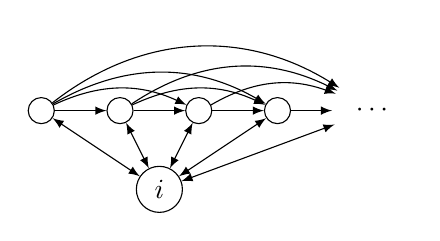
\begin{tikzpicture}[>=latex]
  \node (n1) at (1.5,.5) [shape=circle,draw] {$i$} ;
  \node (n2) at (0,1.5) [shape=circle,draw] {} ;
  \node (n3) at (1,1.5) [shape=circle,draw] {} ;
  \node (n4) at (2,1.5) [shape=circle,draw] {} ;
  \node (n5) at (3,1.5) [shape=circle,draw] {} ;
  \node (n6) at (4.2,1.5) [shape=circle, minimum height=1cm] {$\cdots$} ;

  \draw [<->] (n1) -- (n2);
  \draw [<->] (n1) -- (n3);
  \draw [<->] (n1) -- (n4);
  \draw [<->] (n1) -- (n5);
  \draw [<->] (n1) -- (n6);

  \draw [->] (n2) -- (n3);
  \draw [->] (n3) -- (n4);
  \draw [->] (n4) -- (n5);
  \draw [->] (n5) -- (n6);

  \draw [->] (n2) edge[bend left=25] (n4);
  \draw [->] (n3) edge[bend left=25] (n5);
  \draw [->] (n4) edge[bend left=25] (n6);

  \draw [->] (n2) edge[bend left=30] (n5);
  \draw [->] (n3) edge[bend left=30] (n6);

  \draw [->] (n2) edge[bend left=35] (n6);
\end{tikzpicture}
\end{center}

\end{pf}


We now show that $\cMLRKM + i$ is undecidable by encoding the
$\omega\times\omega$ tiling problem (see~\cite{BGG97}). Following
the idea in~\cite{BS95}, we will construct a \emph{spy point} over the relation
$R_s$; that is, the point of evaluation will have access in one $R_s$-step
to any reachalbe state in the model. The relations $R_u$ and $R_r$
represent moving up and to the right, respectively, from one tile to
the other. We code each type of tile with a fixed propositional
symbol $t_i$. With this encoding we define for each tiling problem
$T$, a formula $\varphi^T$ such that the set of tiles $T$ tiles
$\omega\times\omega$ iff $\varphi^T$ has a model.


\begin{thm}\label{thm:tlmi:und}
The satisfiability problem for $\cMLRKM + i$ is undecidable.
\end{thm}
\begin{pf}
Let $T=\{T_1,\dots,T_n\}$ be a set of tile types. Given a tile type
$T_i$, $u(T_i)$, $r(T_i)$, $d(T_i)$, $l(T_i)$ will represent the
colors of the up, right, down and left edges of $T_i$ respectively.
Define:
$$
\begin{array}{rl}
(\textit{Back}) & i \land \bbox{s}\lnot i \land \ttup{s} \top \land \bbox{s}\ttup{s}i \land \bbox{s}\bbox{s}i\\
(\textit{Empty}) & \bbox{s}\lnot \known \land \bbox{s}\bbox{\dag}\lnot \known \quad \dag \in \{r,u\}\\
(\textit{Spy}) & \bbox{s}\bbox{\dag}\ttup{s}(i \land \ttup{s}(\known \land \lnot\ttup{\dag}\known)) \quad \dag \in \{r,u\}\\
(\textit{Grid}) & \bbox{s}\ttup{\dag} \top \quad \dag \in \{r,u\}\\
(\textit{Func}) & \bbox{s}\bbox{\dag}\ttup{s}\ttup{s}(\known \land \ttup{\dag}\known \land \bbox{\dag}\known) \quad \dag \in \{r,u\}\\
(\textit{Conf}) & \bbox{s}\ttup{u}\ttup{r}\ttup{s}\ttup{s}(\known \land \lnot \ttup{r}\known \land \ttup{u}\known \land \\
& \ \ \ \ttup{r}( \lnot \known \land (\ttup{u}(\known \land \lnot \ttup{r}\known)))\\
(\textit{UR-no-Cycle}) & \bbox{s}\bbox{u}\bbox{r}\lnot \known \land \bbox{s}\bbox{r}\bbox{u}\lnot \known\\
(\textit{URU-no-Cycle}) & \bbox{s}\bbox{u}\bbox{r}\bbox{u}\lnot \known\\
(\textit{Unique}) & \bbox{s} \left( \bigvee_{1\leq i\leq n} t_i \wedge \bigwedge_{1\leq i < j \leq n } (t_i\to \lnot t_j)\right) \\
(\textit{Vert}) & \bbox{s} \bigwedge_{1\leq i\leq n} \left( t_i \to \ttup{u} \bigvee_{1\leq j\leq n,u(T_i)=d(T_j)}  t_j\right) \\
(\textit{Horiz}) & \bbox{s} \bigwedge_{1\leq i\leq n} \left( t_i \to \ttup{r} \bigvee_{1\leq j\leq n,r(T_i)=l(T_j)}  t_j\right) \\
\end{array}
$$

Let the formula $\varphi^T$ be the conjunction of all the above
formulas. We show that $T$ tiles $\omega\times\omega$ iff
$\varphi^T$ is satisfiable.

Suppose $\model,w\models\varphi^T$. Observe that \textit{Back} and
\textit{Spy}, together with \textit{Empty} make $w$ a spy
via $R_s$ (and also force
$R_u$ and $R_r$ to be irreflexive and asymmetric). These $R_s$-accessible
states will represent the tiles. We'll have that $\bbox{s}\psi$
holds at $w$ iff $\psi$ is true at every tile, and
$\ttup{s}\ttup{s}\psi$ holds at tile $v$ iff $\psi$ is
true at some (perhaps the same) tile.
Now, \textit{Grid} states that from every tile there is
another tile moving up (that is, following the $R_u$-relation). The
same holds for the right direction (following the $R_r$-relation).
\textit{Func} (together with \textit{Back} and \textit{Spy}) forces $R_u$ and $R_r$ to be functional. \textit{Conf} ensures that
the tiles are arranged as a grid, once we force $R_u{\circ}R_r$ to be
irreflexive (\textit{UR-Irr}), and we forbid cycles via the $R_uR_rR_r$ pattern (\textit{URU-no-Cycle}).

That completes the description of the grid. The last
three formulas ensure that every tile has a unique type $t_i$, and that the
colors of the tiles match properly. From this, it easily follows
that $\model$ is a tiling of $\omega\times\omega$.

For the converse, suppose $f:\omega\times\omega\to T$ is a tiling of
$\omega\times\omega$. We define the model
$\model=\diam{W,\{R_s,R_u,R_r\},V,\emptyset}$ as follows:
\begin{itemize}
\item $W=\omega\times\omega \cup \{w\}$
\item $R_s=\{(w,v),(v,w)\mid v\in\omega\times\omega\}$  (hence $w$ will act as the spy
point)
\item $R_u=\{((x,y),(x,y+1))\mid x,y\in\omega\}$
\item $R_r=\{((x,y),(x+1,y))\mid x,y\in\omega\}$
\item $V(p)=\{w\}$; $V(t_i)=\{x\mid x\in\omega\times\omega, f(x)=T_i\}$
\end{itemize}
The reader may verify that, by construction,
$\model,w\models\varphi^T$.
\end{pf}

We now turn to the case for $\cMLRKME$. The ideas are similar to the case
of $\cMLRKM + i$ but this time we cannot use the nominal $i$ to makr the
spy point.  On the other hand, we know that the memory is empty when we
start evaluating a formula.


\begin{thm}\label{thm:tlme:inf}
$\cMLRKME$ lacks the finite model property.
\end{thm}

\begin{pf}
Consider the following formulas:
$$
\begin{array}{rl}
(\textit{Back}) & p \land \bbox{r} \lnot p  \land \ttup{r} \top \land \bbox{r}\ttup{r} (\known \land p) \\
%&$``The root is irreflexive, and in symmetric relation with all its (nonempty) successors.''$\\
(\textit{Spy}) & \bbox{r}\bbox{r}( \lnot p \to \ttup{r} (\known \land p \land \ttup{r} ( \known \land \lnot \ttup{r} ( \known \land \lnot p))))\\
%&$``A 2-step successor is a 1-step successor, with a non-symmetric relation between them.''$\\
(\textit{Irr}) & \lnot \ttup{r} ( \lnot p \land \ttup{r} ( \lnot p \land \known)))\\
%&$``All successors are irreflexive.''$\\
(\textit{Succ}) & \bbox{r}\ttup{r} \lnot p \\
%&$``All successors have a successor different from the root.''$\\
(\textit{No-3cyc}) & \lnot \ttup{r}   \ttup{r} ( \lnot \known \land \ttup{r} ( \lnot \known \land \ttup{r} ( \known \land \lnot p)))\\
%&$``There are no cycles of 3 elements between successors of the root.''$\\
(\textit{Tran}) & \bbox{r} ( \lnot p \to \ttup{r} ( \known \land p \land \bbox{r} ( \lnot p \land \lnot \known \to \ttup{r}( \known \land p \land \\
& \ \ \ \ttup{r} ( \known \land \lnot p \land  \ttup{r}(\known \land \lnot p) )))))\\
%&$``Every pair of successors $u$ and $v$ are related (either $uRv$ or $vRu$).''$\\
\end{array}
$$

Let $\textit{Inf}$ be $\textit{Back} \land \textit{Spy} \land
\textit{Irr} \land \textit{Succ} \land \textit{no-3cyc} \land
\textit{Tran}$, and let $\model=\diam{W, R, V, \emptyset}$.
The proof that $\model$ is infinite if $\model, w \models \textit{Inf}$ is similar to the proof of Theorem~\ref{thm:tlmi:inf}.
Instead of using  $i$ to identify the spy point we now use
$p$ and $\known$. $\known$ is needed to distinguish the spy point
from other points where $p$ might hold.


Notice that \textit{Back}, \textit{Spy}, \textit{Succ}, and
\textit{no-3cyc} are very similar to the ones in the proof of
Theorem~\ref{thm:tlmi:inf}, \textit{Irr} forces $R$ to be
irreflexive and \textit{Tran} says that every pair of successors $u$
and $v$ are related (either $R(u,v)$ or $R(v,u)$), and this together with
the other formulas, implies that $R$ is transitive.

%
%Suppose $\model, w \models \textit{Inf}$. Let $B = \{b \in W \mid
%wRb\}$. Because $\textit{Back}$ is satisfied, $w \not \in B$, $B
%\not= \emptyset$ and for all $b \in B$, $bRw$. Because
%$\textit{Spy}$ is satisfied, if $a \not= w$ and $a$ is a successor
%of an element of $B$ then $a$ is also an element of $B$. As
%$\textit{Irr}$ is satisfied at $w$, every state in $B$ is
%irreflexive. As $\textit{Succ}$ is satisfied at $w$, every point in
%$B$ has a successor distinct from $w$. As $\textit{3cyc}$ is
%satisfied, there cannot be $3$ different elements in $B$ forming a
%cycle, and this sentence together with $\textit{Tran}$ force $R$ to
%transitively order $B$.
%
%It follows that $B$ is an unbounded strict partial order, hence
%infinite, and so is $W$.
\end{pf}


In a similar way, we can encode the $\omega
\times \omega$ tiling problem to show that satisfiability in
$\cMLRKME$ is undecidable.

\begin{thm}\label{thm:tlme:und}
The satisfiability problem for $\cMLRKME$ is undecidable.
\end{thm}
\begin{pf}
The formula $\varphi_T$ needed for the encoding of a tiling problem
$T$ in this case is the conjunction of the following:
$$
\begin{array}{rl}
(\textit{Back}) & p \land \bbox{s}\lnot p \land \ttup{s} \top \land \bbox{s}\ttup{s}(\known \land p) \land \bbox{s}\bbox{s}(\known \land p)\\
(\textit{Spy}) & \bbox{s}\bbox{\dag}(\lnot p \land \ttup{s}(\known \land p \land \ttup{s}(\known \land \lnot\ttup{\dag}\known))) \quad \dag \in \{r,u\}\\
(\textit{Grid}) & \bbox{s}\ttup{\dag} \top \quad \dag \in \{r,u\}\\
(\textit{Func}) & \bbox{s}\bbox{\dag}\ttup{s}\ttup{s}(\known \land \ttup{\dag}\known \land \bbox{\dag}\known) \quad \dag \in \{r,u\}\\
(\textit{Conf}) & \bbox{s}\ttup{u}\ttup{r}\ttup{s}\ttup{s}(\known \land
\lnot \ttup{r}\known \land \ttup{u}\known \land \\
& \ \ \ \ttup{r}\ttup{u}(\known \land \lnot \ttup{r}\known))\\
(\textit{URU-no-Cycle}) & \bbox{s}\bbox{u}\bbox{r}\lnot \known \land \bbox{s}\bbox{r}\bbox{u}\lnot \known\\
(\textit{URU-no-Cycle}) & \bbox{s}\bbox{u}\bbox{r}\bbox{u}\lnot \known\\
(\textit{Unique}) & \bbox{s} \left( \bigvee_{1\leq i\leq n} t_i \wedge \bigwedge_{1\leq i < j \leq n } (t_i\to \lnot t_j)\right) \\
(\textit{Vert}) & \bbox{s} \bigwedge_{1\leq i\leq n} \left( t_i \to \ttup{u} \bigvee_{1\leq j\leq n,u(T_i)=d(T_j)}  t_j\right) \\
(\textit{Horiz}) & \bbox{s} \bigwedge_{1\leq i\leq n} \left( t_i \to
\ttup{r} \bigvee_{1\leq j\leq n,r(T_i)=l(T_j)}  t_j\right)
\end{array}
$$
%Suppose $\model,w\models\varphi^T$. Observe that (\textit{Back}) and
%(\textit{Spy}) impose $w$ to be a spy point over all its
%$S$-accessible states of $\model$ (and also force $U$ and $R$ to be
%irreflexive and asymmetric). These $S$-accessible states will be the
%tiles. From this it follows that $[S]\psi$ holds at $w$ iff $\psi$
%is true at every tile. Additionally, $\diam{S}\diam{S}\psi$ holds at
%tile $v$ iff $\psi$ is true at some tile (maybe the same one).
%
%Taking the above points into account, one can establish the
%following. (\textit{Grid}) states that from every tile there is
%another tile moving up (that is, following the $U$-relation). The
%same holds for the right direction (following the $R$-relation).
%(\textit{Func}) forces that $U$ and $R$ are both functionals, given
%that (\textit{Back}) and (\textit{Spy}) guarantee irreflexivity and
%asymmetry of $U$ and $R$ respectively. (\textit{Conf}) imposes that
%the tiles are arranged in a grid pattern. To make its job,
%(\textit{Conf}) needs the composed relation $U\circ R$ to be
%irreflexive, and to avoid a cycle with the $URU$ pattern. This job
%is done by (\textit{UR-Irr}) and (\textit{URU-noCycle})
%respectively.
%
%All the formulas we discuss up to now configure the grid. The last
%three ensure that every tile has a unique type $t_i$, and that the
%colors of the tiles match properly. From this, it easily follows
%that $\model$ is a tiling of $\omega\times\omega$.
%
%For the converse, suppose $f:\omega\times\omega\to T$ is a tiling of
%$\omega\times\omega$. We define the model
%$\model=\diam{W,\{S,U,R\},V,\emptyset}$ as follows:
%\begin{itemize}
%\item $W=\omega\times\omega \cup \{w\}$
%\item $S=\{(w,v),(v,w)\mid v\in\omega\times\omega\}$  (hence $w$ will act as the spy
%point)
%\item $U=\{((x,y),(x,y+1))\mid x,y\in\omega\}$
%\item $R=\{((x,y),(x+1,y))\mid x,y\in\omega\}$
%\item $V(p)=\{w\}$; $V(t_i)=\{x\mid x\in\omega\times\omega, f(x)=T_i\}$
%\end{itemize}
%The reader may verify that, by construction,
%$\model,w\models\varphi^T$.
%
\end{pf}

\subsection{The Undecidable $\cMLRK$ and $\cMLRKE$}

From the undecidability of $\cMLRKME$, we can easily conclude the
undecidability of $\cMLRK$ and $\cMLRKE$.

\begin{thm}
$\cMLRKE$ lacks the finite model property and it is undecidable.
\end{thm}

\begin{pf}
Straightforward from the effective translation given as a result of
$\cMLRKME \leq \cMLRKE$ (Theorem~\ref{thm:four-le-two}) and
Theorems~\ref{thm:tlme:inf} and~\ref{thm:tlme:und}.
\end{pf}

To prove failure of the finite model property for the case $\cMLRK$
we first notice that the following lemma is easy to establish (we only
state it for the mono-modal case; a similar result is true in the
multi-modal case).
Failure of the finite model property is then a direct consequence.

\begin{lem}\label{lem:boxes}
Let $\varphi$ be a formula of modal depth $d$. If {\em
$\diam{W,R_r,V,S},w\models$} \linebreak {\em
$\left(\bigwedge_{i=0}^d [r]^i \lnot \known\right) \wedge \varphi$}
then $\diam{W,R_r,V,\emptyset},w\models \varphi$.
\end{lem}

\begin{cor}
{\em $\cMLRK$} lacks the finite model property.
\end{cor}

\begin{pf}
Using Lemma~\ref{lem:boxes}, one can easily see that the formula
$\left(\bigwedge_{i=0}^4 [r]^i \lnot
\known\right) \wedge \textit{Inf}$, where $\textit{Inf}$ is the one in the proof of
Theorem~\ref{thm:tlme:inf}, forces an infinite model.
\end{pf}



\begin{cor}
The satisfiability problem for {\em $\cMLRK$} is undecidable.
\end{cor}
%
\begin{pf}
Using the idea of Lemma~\ref{lem:boxes} and the formula $\varphi^T$
in the proof of Theorem~\ref{thm:tlme:und}, we can obtain a formula
$\psi$ such that if $\model,w\models\psi$ then $\model$ is a tiling
of $\omega \times \omega$. For the converse, we can build exactly
the same model as in the proof of Theorem~\ref{thm:tlme:und} and
check that it satisfies $\psi$.
\end{pf}
